\documentclass[]{article}

\usepackage{geometry}
\geometry{
	a4paper,
	total={170mm,257mm},
	left=20mm,
	top=20mm,
}

\usepackage[utf8]{inputenc}
\usepackage[english,russian]{babel}
\usepackage{pscyr}
\usepackage{gensymb}
\usepackage{amsmath}
\usepackage{multicol}
\usepackage]{epstopdf}
\usepackage{graphicx}
\usepackage{tikz}
\begin{document}
%\begin{multicols}{2}	
	
Уравнения генератора
\begin{subequations}
\begin {equation}
M_j = T_j P_{nom}
\end {equation}
\begin {equation}
M_j\frac{ds}{dt} = (\frac{P_t}{1+s} - \frac{P}{1+s_v} - sK_{demp})
\end {equation}
\begin {equation}
\frac{d\delta}{dt} = \omega_0s
\end {equation}
\end{subequations}

\begin{equation}
E_{qenom}=\frac{U^4_{nom}+U^2_{nom}Q_{nom}(x_d+x_q)+S^2_{nom}x_dx_q}{U_{nom}\sqrt{U^4_{nom}+2U^2_{nom}Q_{nom}x_q+S^2_{nom}x^2_q}}
\end{equation}


Президент США Дональд Трамп может вернуться к вопросу о Парижском соглашению по климату. Об этом заявил французский лидер Эмманюэль Макрон, сообщает Reuters со ссылкой на газету Le Journal du Dimanche.

«[Трамп] сказал мне, что он попытается найти решение данного вопроса в ближайшие месяцы», — сказал Макрон. — «Мы обсудили детали того, что поможет ему вернуться к Парижскому соглашению».

Трамп объявил о выходе из Парижского соглашения 1 июня. По его словам, оно невыгодно для США, так к 2025 году при исполнении положений договора Америка потеряет 2,7 млн рабочих мест. Однако американский лидер заявил, что Вашингтон будет вести переговоры по корректировке соглашения, чтобы оно было справедливым для граждан США. Трамп подчеркнул, что Соединенные штаты не будут соблюдать «необязательные» пункты документа с 1 июня.

Подробнее на РБК:
http://www.rbc.ru/rbcfreenews/596ab7089a794775306ec0ab?from=newsfeed

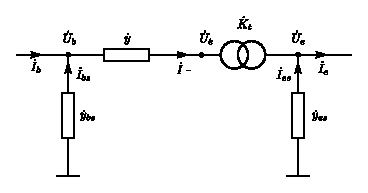
\includegraphics{C:/tmp/piline}   

\begin {center}
\begin{tabular} {c c r}

\begin{tikzpicture}[sibling distance=10em,
every node/.style = {shape=rectangle, rounded corners,
	draw, align=center,
	top color=white, bottom color=blue!20}]]
\node {$x^a$}
child { node {$a$}  }
child { node {$x$}  };
\end{tikzpicture}

&

\begin{tikzpicture}[sibling distance=10em,
every node/.style = {shape=rectangle, rounded corners,
	draw, align=center}]]
\node {$*$}
child { node {$a$}      }
child { node {$x^{a-1}$ } 
	child {node {$a-1$} }
	child {node {$x$} } }
child { node {$x'$} };
\end{tikzpicture}
\end{tabular}
\end{center}

\end{document}
